\begin{sagesilent}
import matplotlib.pyplot as plt
import numpy as np

d = load("http://pubdata.sage.wikifm.org/lab2-exp-data/misura-c.sobj", verbose=False)
m1 = d["m1"]
m2 = d["m2"]
speed = d["speed"]

diff = []
sp = []
diff2 = []
sp2 = []
for i in range(0,len(m1)):
    if (m2[i]-m1[i]) > 0:
        diff.append(m2[i]-m1[i])
        sp.append(speed[i]*6.28)
    else:
        diff2.append(m1[i]-m2[i])
        sp2.append(speed[i]*6.28)

var('m, q')
model(x) = m*x+q
dataprime = [(sp[i], diff[i]) for i in range(0, len(sp))]
fit = find_fit(dataprime, model, solution_dict = True)

def plot_experiment(m, q):
    plt.clf()
    plt.plot(sp, diff, '.k')
    plt.plot(sp2, diff2, '.r')
    xin = np.arange(min(sp)*0.8, max(sp)*1.2, 100)
    yin = m*xin+q
    plt.xlabel(r"$\omega (rad/s)$")
    plt.ylabel(r"$\Delta s (\mu m)$")
    plt.plot(xin, yin, "g-")
    plt.grid(True)
    plt.savefig("grafici/C/dati.png", dpi=300)
    
d = 13480
f = 252
b = 220
a = (b+d)*f/(b+d-f)
\end{sagesilent}


\chapter{Misura della velocità della luce}

L'obiettivo del nostro esperimento è misurare la velocità della luce $c$.

L'apparato di misurazione consiste principalmente in:
\begin{itemize}
 \item Un laser Elio-Neon ($\lambda=632$ nm).
 \item Uno specchio rotante a velocità angolare regolabile.
 \item Due lenti convergenti, di lunghezza focale $l_1 = 48mm$ e $l_2 = 252 mm$.
 \item Un microscopio con beam splitter e micrometro.
\end{itemize}

Lo specchio rotante viene fatto girare con velocità angolare $\omega_1$ in senso orario e $\omega_2$ in senso antiorario. Queste velocità angolari sono identiche nella maggior parte dei casi, e la loro differenza è trascurabile.

Chiamando $s_{cw}$ e $s_{ccw}$ rispettivamente le misure del punto luminoso prese a micrometro con specchio rotante in senso orario e antiorario, per come è orientata la strumentazione il numero
$$\Delta s = s_{cw} - s_{ccw}$$
deve essere positivo.

Purtroppo però non è questo il caso per qualche misura presa in mattinata, per ragioni sconosciute e che non siamo riusciti a riprodurre. Questi dati sono esclusi dalla misurazione in quanto evidenti errori, e sono mostrati in rosso nel grafico seguente
I dati sono molti, dunque forniamo qui soltanto una visione grafica, e lasciamo la tabella come allegato.

\section{Analisi dati}

\begin{sagesilent}
at = 4*a*d^2/(d+b)
plot_experiment(fit[m], fit[q]) 
\end{sagesilent}


Chiamiamo $D = \sage{d}$mm il cammino geometrico della luce per tornare allo specchio rotante, ovvero il doppio della distanza specchio rotante/specchio fisso; $A$ la distanza del punto di convergenza del fascio laser dalla lente $l_2$ e $B$ la distanza tra $l_2$ e lo specchio rotante. 

Per calcolare con precisione $A$, conoscendo la distanza focale di $l_2$, la ricaviamo dalla formula dei punti coniugati:
$$A=\frac{(B+D)f}{B+D-f} = \sage{n(a, digits=4)} \text{mm}$$


Per calcolare $c$, dobbiamo interpolare i dati presi nel modo seguente:
$$\Delta s = \frac{\tilde{A}}{c}\omega$$
ove
$$\tilde{A} = \frac{4*A*D^2}{D+B}$$


La funzione che ci permetterà di calcolare $c$ è ora banale, e con in nostri dati vale:

$$c = \frac{\tilde{A}}{m} = \sage{n(at/fit[m], digits=4)} \text{m/s}$$

\begin{center}
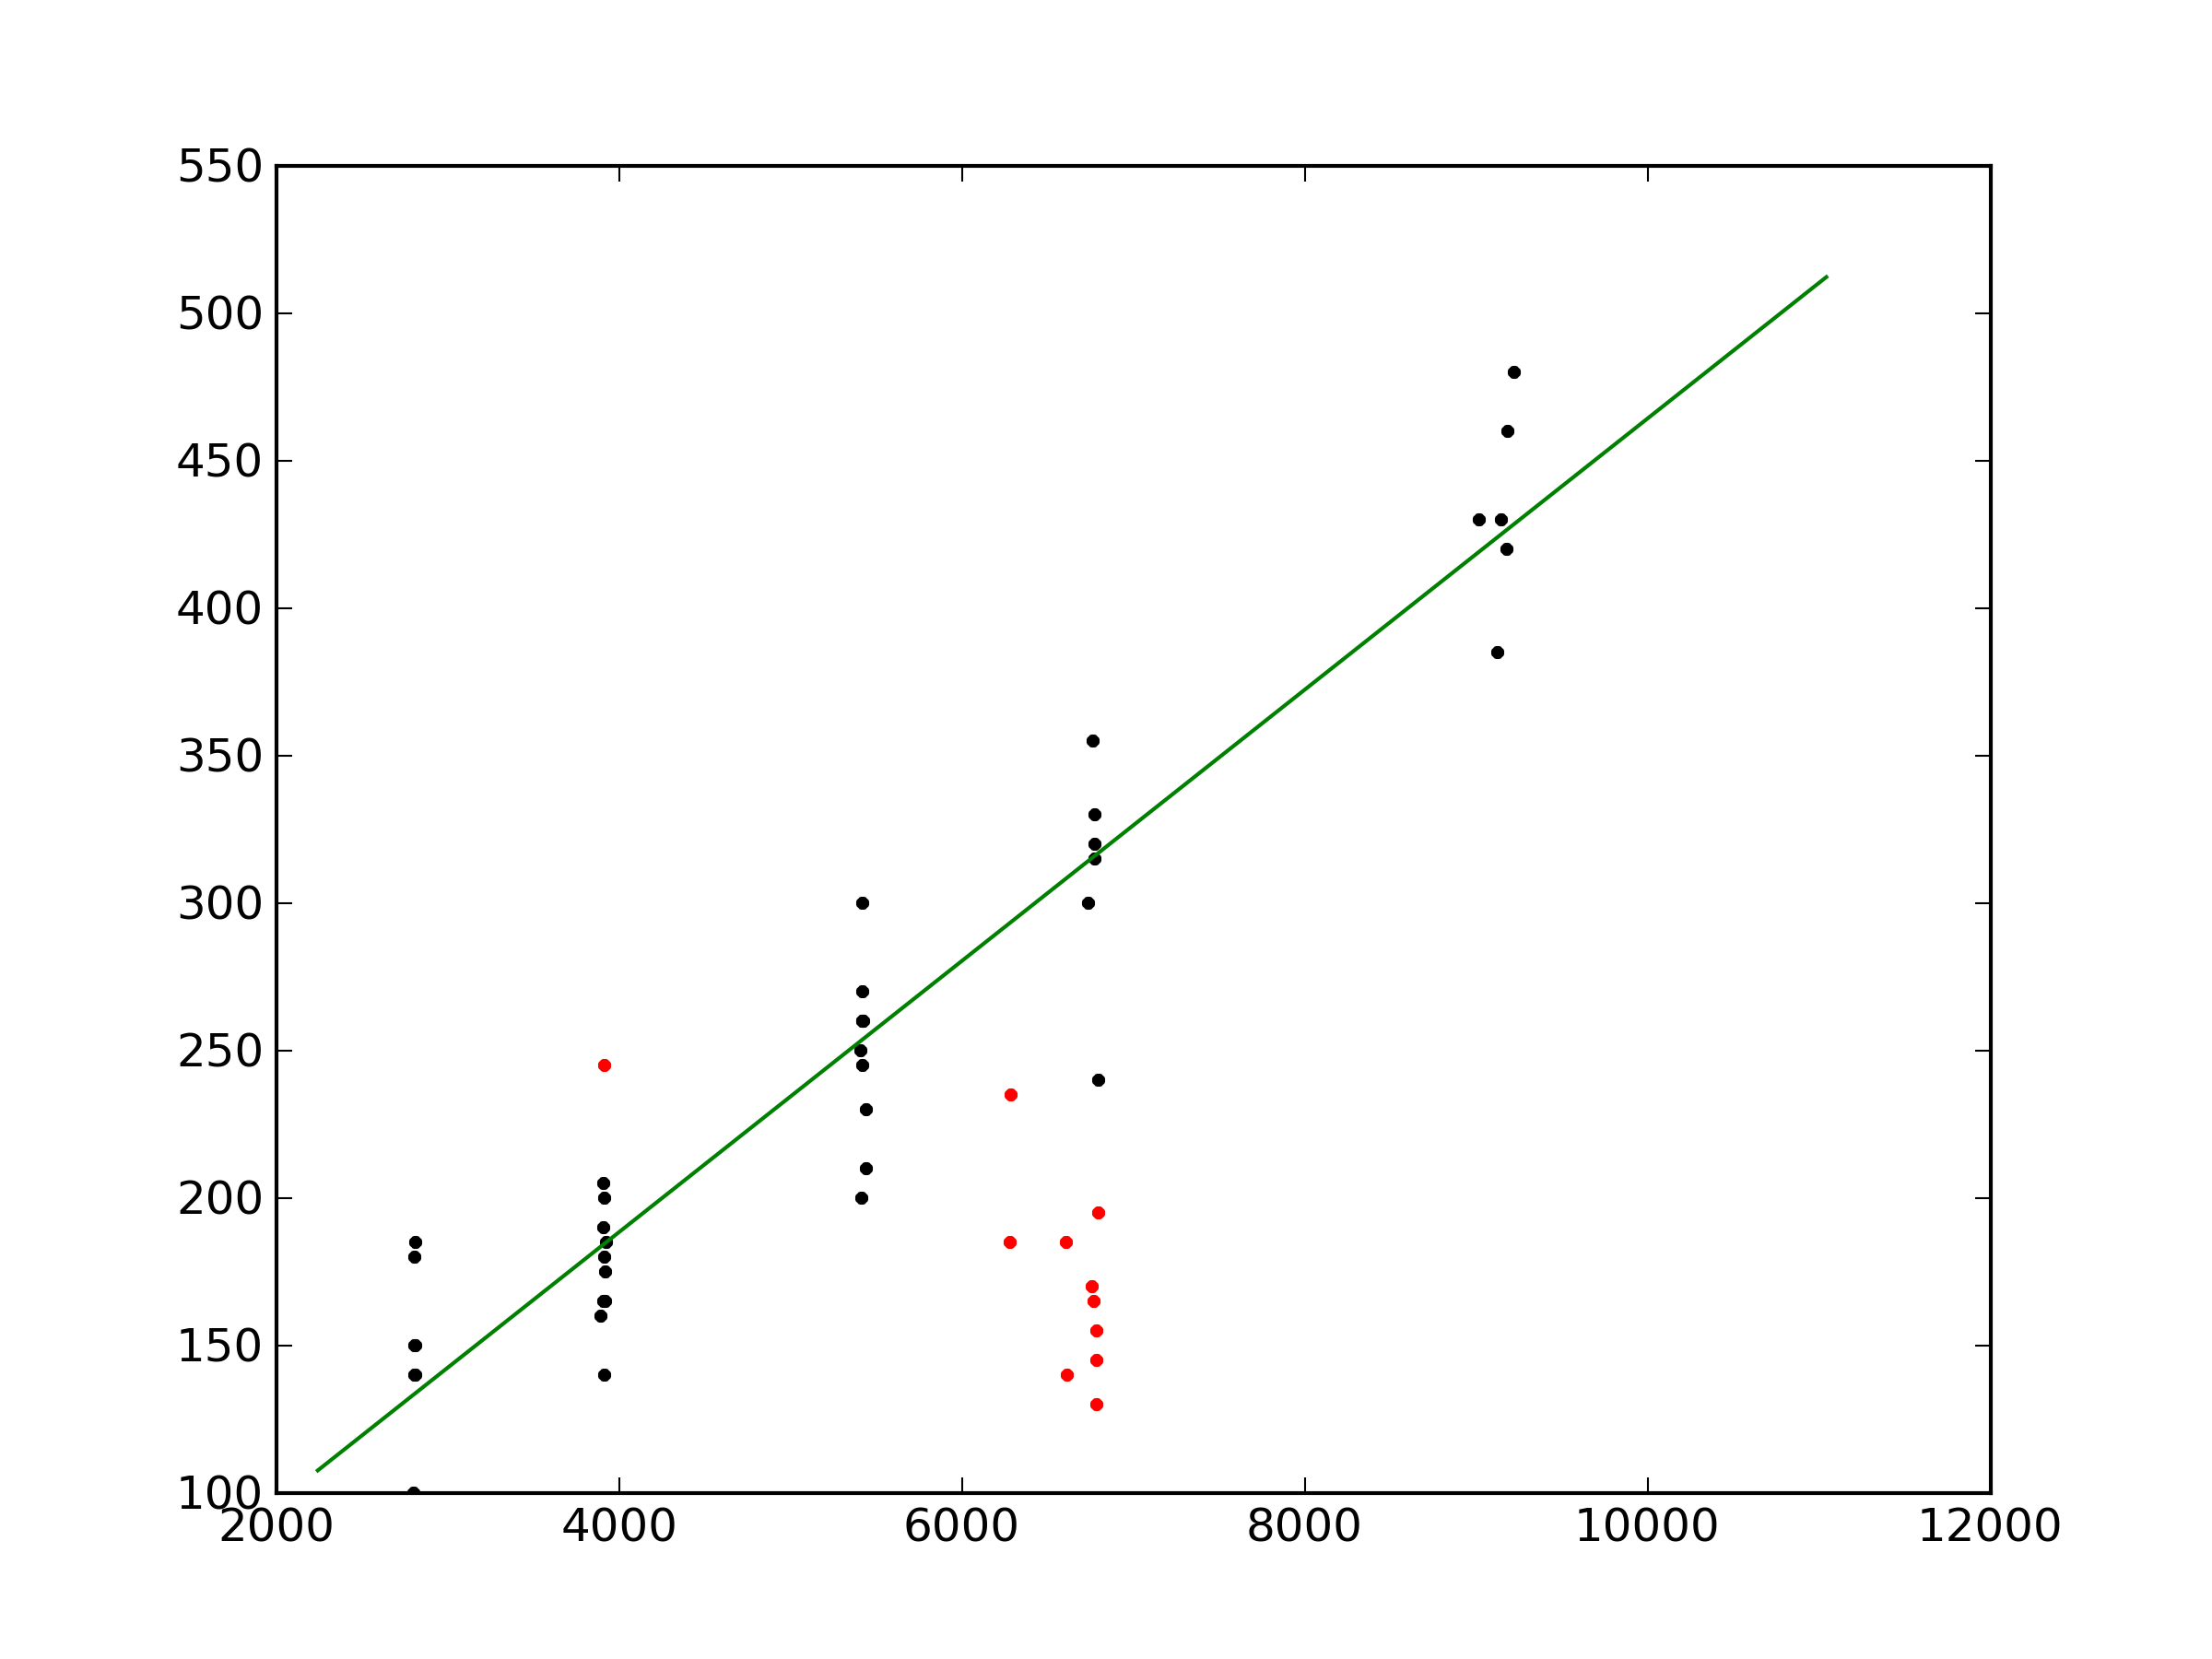
\includegraphics[scale=0.75]{grafici/C/dati.png}
\end{center}

Valutiamo la bontà del nostro fit con il test del $\chi^2$. L'errore è evidentemente maggiore dell'errore dovuto alla precisione strumentale (5 $\mu$m), e dunque utilizzeremo la stima a posteriori degli errori. Con questi dati otteniamo:

\begin{sagesilent}
# Chi quadro
def funct(x):
    return fit[m]*x+fit[q]

chi = 0
for i in range(0,len(diff)):
    teo = funct(sp[i])
    chi += (diff[i]-teo)^2/teo
    
chirid = chi/(len(diff)-3)
\end{sagesilent}

$$\chi^2 = \sage{n(chi, digits=4)}$$
$$\tilde{\chi}^2 = \sage{n(chirid, digits=4)}$$

\section{Allegato: dati}
\begin{sagesilent}
def stampa_dati(vel, deltas):
  s = r"\begin{tabular}{c|c}"
  s += r"$\omega$ ($rad/s$) & $|\Delta s|$ ($\mu$m) ($\pm5\mu m$) \\"
  s += r"\midrule"
  for i in range(0, len(vel)):
    s += "%d & %d \\\\" % (vel[i], deltas[i])
  s += r"\end{tabular}"
  return s
\end{sagesilent}

\begin{center}
 \sagestr{stampa_dati(sp, diff)}
\end{center}
Dati scartati:
\begin{center}
 \sagestr{stampa_dati(sp2, diff2)}
\end{center}
